\documentclass{article}
\usepackage[english]{babel}
\usepackage[letterpaper,top=2cm,bottom=2cm,left=3cm,right=3cm,marginparwidth=1.75cm]{geometry}
\usepackage{lmodern}
\usepackage[T1]{fontenc}

% Useful packages
\usepackage{amsmath}
\usepackage{amsfonts}
\usepackage{graphicx}
\usepackage[colorlinks=true, allcolors=blue]{hyperref}
\usepackage{booktabs}
\usepackage{subcaption}
\usepackage{microtype}
\usepackage{placeins} % \FloatBarrier
% algorithms
\usepackage{algorithm}
\usepackage{algpseudocode}
\algdef{SE}[PARFOR]{ParFor}{EndParFor}[1]{\textbf{parfor} $#1$ \textbf{do}}{\textbf{end parfor}}
% bibliography
\usepackage{authblk}
\usepackage{csquotes}
%\usepackage[style=numeric, backend=bibtex]{biblatex}
%\addbibresource{references.bib}
% tikz
\usepackage{tikz}
\usetikzlibrary{positioning, arrows.meta, fit, shapes.geometric, calc, shadows}
% Author notes are suppressed in the submission version.  The commands remain
% defined because Section 1 is intentionally kept verbatim.
\newcommand{\mg}[1]{}
\newcommand{\mginline}[1]{}
\newcommand{\al}[1]{}
\newcommand{\alinline}[1]{}

\title{A Spectrally Calibrated Geometry-Conditioned Neural IETI-DP Preconditioner}
\date{}
\author[1]{Massimiliano Ghiotto}
\author[2]{Alessandro Lucantonio}
\affil[1]{Department of Mathematics, University of Pavia}
\affil[2]{Department of Mechanical and Production Engineering, Aarhus University}



% User defined commands
\newcommand{\vect}[1]{\boldsymbol{#1}}
\newcommand{\R}{\mathbb{R}}
\newcommand{\N}{\mathbb{N}}
\newcommand{\skel}{\Gamma} % skeleton (interface) index set
\DeclareMathOperator{\spann}{span}
\newcommand{\npatch}{K} % number of patches

% -----------------------------------------------------------------------
% Notation macros
% -----------------------------------------------------------------------
% Domains
\newcommand{\refdom}{\widehat{\Omega}}            % reference/parameter domain
\newcommand{\patchdom}[1]{\Omega_{#1}}            % k-th patch physical domain

% Basis functions
\newcommand{\bsuni}[2]{\widehat{b}_{#1,#2}}      % univariate B-spline
\newcommand{\Bref}[2]{\widehat{B}_{#1,#2}}       % reference tensor-product B-spline
\newcommand{\Bphy}[2]{B_{#1,#2}}                  % physical (push-forward) basis function
\newcommand{\Bloc}[2]{B^{(#1)}_{#2}}              % local patch basis (patch index, DOF index)
\newcommand{\Rnurbs}[2]{\widehat{R}_{#1,#2}}     % NURBS (rational) basis

% Function spaces
\newcommand{\Shat}[1]{\widehat{\mathcal{V}}_{#1}} % reference spline space (uni- or multivariate)
\newcommand{\Vglo}{\mathcal{V}_h}                  % global conforming IGA space
\newcommand{\Vloc}[1]{\mathcal{V}_{#1}}            % local patch IGA space
\newcommand{\Vprod}{\mathcal{V}_h^{\Pi}}           % product (broken) space

% Geometry maps
\newcommand{\gmap}{\mathcal{F}}                   % geometry map (single-patch or global context)
\newcommand{\gmapk}[1]{\mathcal{F}_{#1}}         % patch-k geometry map

% Global stiffness and load
\newcommand{\Aglo}{A}                             % global stiffness matrix
\newcommand{\fglo}{\vect{f}}                      % global load vector
\newcommand{\uglo}{\vect{u}}                      % global solution vector

% Local stiffness and load
\newcommand{\Aloc}[1]{A_{#1}}                    % local stiffness matrix
\newcommand{\Aaug}[1]{\widetilde{A}_{#1}}        % augmented (IETI) stiffness
\newcommand{\floc}[1]{\vect{f}_{#1}}             % local load vector
\newcommand{\faug}[1]{\widetilde{\vect{f}}_{#1}} % augmented load vector

% Jump (continuity) matrices -- J to avoid clash with basis functions B
\newcommand{\Jloc}[1]{J_{#1}}                    % local jump matrix
\newcommand{\Jfull}{J}                            % global jump operator
\newcommand{\Jskel}[1]{\widehat{J}_{#1}}         % jump restricted to skeleton DOFs
\newcommand{\Jaug}[1]{\widetilde{J}_{#1}}        % augmented jump (IETI)

% Schur complements
\newcommand{\Sloc}[1]{S_{#1}}                    % local Dirichlet Schur complement
\newcommand{\Snn}{\mathcal{S}_{\theta}}          % neural Schur operator

% Primal constraints and basis
\newcommand{\Cloc}[1]{C_{#1}}                    % primal constraint matrix
\newcommand{\Psik}[1]{\Psi_{#1}}                 % primal energy-minimising basis
\newcommand{\nprim}{n_\Pi}                        % number of primal DOFs

% Interface (dual) system
\newcommand{\Fschur}{F}                           % interface Schur operator
\newcommand{\gschur}{\vect{g}}                    % interface right-hand side

% Preconditioners
\newcommand{\Psd}{M_{sD}^{-1}}                   % scaled Dirichlet preconditioner
\newcommand{\Pneural}{M_{\theta}^{-1}}            % neural preconditioner

% Neural architecture
\newcommand{\dv}{d_v}                             % latent dimension of Transformer

% Multiplicity scaling
\newcommand{\Dmult}[1]{D_{#1}}                   % multiplicity-weighted diagonal

% Free local degrees of freedom of patch k (skeleton + interior)
\newcommand{\dofset}{\mathcal{N}}                % index set of free local dofs

% Local and augmented solutions
\newcommand{\uloc}[1]{\vect{u}_{#1}}             % local patch solution
\newcommand{\uaug}[1]{\widetilde{\vect{u}}_{#1}} % augmented local solution (IETI)
\newcommand{\lagmult}{\vect{\lambda}}             % Lagrange multipliers

% -----------------------------------------------------------------------

% Theorem environments
\usepackage{amsthm}
\theoremstyle{plain}
\newtheorem{ass}{Assumption}
\newtheorem{lemma}{Lemma}
\newtheorem{prop}{Proposition}
\newtheorem{theorem}{Theorem}
\newtheorem{df}{Definition}
\newtheorem{rmk}{Remark}
\newtheorem{cor}{Corollary}
\numberwithin{equation}{section}


\begin{document}
\maketitle
% \tableofcontents

%%%%%%%%%%%%%%%%%%%%%%%%%%%%%%%%%%%%%%%%%
%% Abstract
%%%%%%%%%%%%%%%%%%%%%%%%%%%%%%%%%%%%%%%%%
\begin{abstract}
    We introduce a geometry-conditioned neural preconditioner for the dual-primal
    isogeometric tearing and interconnecting (IETI-DP) method.  A Transformer maps
    patch geometry to a symmetric positive-definite approximation of the local
    Dirichlet Schur operator.  During reusable setup, at most four inaccurate local
    generalized eigenmodes per patch are calibrated and an adaptive Ritz space
    corrects a bounded number of global interface modes.  Large interfaces use a
    residual-certified matrix-free block-Krylov construction; interfaces of order
    at most 16 use a deterministic setup-time analysis.  The final dense operators
    are cached, so no neural inference
    or adaptive construction occurs during a solve.  Separate models are trained
    for six degree--refinement pairs; patch-subdivision experiments use an
    explicitly subdivision-augmented geometry dataset.  Across 16 distinct Yeti
    and teapot configurations, the proposed method has strictly fewer PCG
    iterations and lower solve-only mean time than unmodified scaled-Dirichlet
    IETI-DP.  Over 30 serial repetitions, the measured speedup ranges from
    $1.13\times$ to $2.68\times$.  At $(p,r)=(2,2)$, the Yeti comparison
    changes from 14 iterations and $6.519$ ms to 9 iterations and $4.467$ ms;
    the teapot comparison changes from 19 iterations and $1.415$ ms to 8
    iterations and $0.700$ ms.  A second model trained on 214 non-teapot patch
    operators reduces a whole-family held-out teapot from 19 to 12 iterations
    and from $1.392$ to $0.979$ ms.  Applying the same global correction to the
    classical preconditioner is reported as an attribution control and is often
    stronger on the teapot.  All claims concern repeated solve-only time: model
    inference, local calibration, Ritz construction, factorization, and caching
    are setup and remain recorded in the released artifacts.
\end{abstract}

\noindent\textbf{Keywords:} isogeometric analysis; IETI-DP; domain
decomposition; neural preconditioning; Schur complement; geometry transfer.

%%%%%%%%%%%%%%%%%%%%%%%%%%%%%%%%%%%%%%%%%
%% Section
%%%%%%%%%%%%%%%%%%%%%%%%%%%%%%%%%%%%%%%%%
\section{Preliminaries} \label{sec:preliminaries}

In this section we fix the notation and recall the principal concepts needed in the
remainder of the paper. We first define B-splines and the associated
isogeometric spaces (Section~\ref{subsec:bsplines}), state the model problem and
its multipatch discretization (Section~\ref{subsec:model}), and summarize the
dual-primal Isogeometric Tearing and Interconnecting (IETI-DP) method
(Section~\ref{subsec:ieti}) \cite{kleiss2012ieti}.

%%%%%%%%%%%%%%%%%%%%%%%%%%%%%%%%%%%%%%%%%
\subsection{B-splines and isogeometric spaces} \label{subsec:bsplines}

Given integers $m, p > 0$, a knot vector is a non-decreasing sequence
$\Xi := \{0 = \xi_1 \le \dots \le \xi_{m+p+1} = 1\}$, which we take \emph{open},
i.e.\ $\xi_1 = \dots = \xi_{p+1} = 0$ and $\xi_{m+1} = \dots = \xi_{m+p+1} = 1$.
The Cox--de Boor recursion~\cite{de1978practical} defines the univariate B-spline
basis functions $\bsuni{i}{p} : [0,1] \to \R$, $i = 1, \dots, m$:
\begin{equation*}
    \bsuni{i}{0}(\eta) =
    \begin{cases}
        1 & \text{if } \xi_i \le \eta < \xi_{i+1}, \\
        0 & \text{otherwise},
    \end{cases}
    \qquad
    \bsuni{i}{p}(\eta) =
    \frac{\eta - \xi_i}{\xi_{i+p} - \xi_i}\, \bsuni{i}{p-1}(\eta)
    + \frac{\xi_{i+p+1} - \eta}{\xi_{i+p+1} - \xi_{i+1}}\, \bsuni{i+1}{p-1}(\eta),
\end{equation*}
with the convention $0/0 = 0$; an interior knot of multiplicity $\kappa$ yields
$C^{p-\kappa}$ continuity~\cite{cottrell2009isogeometric}. The constructed basis functions span the univariate
spline space $\Shat{p} := \spann\{\bsuni{i}{p}\}_{i=1}^{m}$.
Multivariate B-splines are constructed with tensor products; on $\refdom := (0,1)^d$,
with a degree $p_l$ and an open knot vector per direction $l = 1, \dots, d$, we
set $\Bref{\vect{i}}{\vect{p}}(\vect{\eta}) := \prod_{l=1}^{d}
    \bsuni{i_l}{p_l}(\eta_l)$ for $\vect{\eta} \in \refdom$. Defining a
colexicographical reordering into a single index $i = 1, \dots, n$, with
$n := \prod_{l=1}^{d} m_l$, gives the reference function space $\Shat{\vect{p}} :=
    \spann\{\Bref{i}{\vect{p}}\}_{i=1}^{n}$.

The physical domain $\Omega \subset \R^{D}$ ($D \ge d$) is the image
$\Omega = \gmap(\refdom)$ of a \emph{geometry map}
$\gmap = \sum_{i=1}^{n} \vect{P}_i\, \Bref{i}{\vect{p}} \in
    [\Shat{\vect{p}}]^{D}$ with control points $\vect{P}_i \in \R^{D}$.
We assume that the geometry map is invertible with full-rank Jacobian $J_{\gmap} = D\gmap$.
For $D = d$ the domain is planar or volumetric; for $D > d$ it is a manifold
(e.g.\ a surface in $\R^3$) and $\nabla_\Omega$ denotes the tangential gradient,
which takes values in the tangent space $\operatorname{range}(J_{\gmap})$.  Writing
$\widehat u := u \circ \gmap$, the chain rule gives
$\nabla_{\vect\eta}\widehat u = J_{\gmap}^{\top}\nabla_\Omega u$.  Because
$\nabla_\Omega u \in \operatorname{range}(J_{\gmap})$, this relation determines
$\nabla_\Omega u$ uniquely:
\begin{equation}
    \nabla_\Omega u
    = J_{\gmap}\bigl(J_{\gmap}^{\top} J_{\gmap}\bigr)^{-1}
      \nabla_{\vect\eta}\widehat u
    = \bigl(J_{\gmap}^{\dagger}\bigr)^{\top}\nabla_{\vect\eta}\widehat u,
    \qquad
    J_{\gmap}^{\dagger} := \bigl(J_{\gmap}^{\top} J_{\gmap}\bigr)^{-1}
        J_{\gmap}^{\top},
    \label{eq:tangential-gradient}
\end{equation}
where $J_{\gmap}^{\dagger}$ is the Moore--Penrose \emph{left} inverse of the
tall, full-column-rank matrix $J_{\gmap} \in \R^{D\times d}$; the right inverse
$J_{\gmap}^{\top}(J_{\gmap}J_{\gmap}^{\top})^{-1}$ does not exist for $D>d$, since
$J_{\gmap}J_{\gmap}^{\top}\in\R^{D\times D}$ has rank $d<D$.  For $D=d$,
\eqref{eq:tangential-gradient} reduces to the familiar
$\nabla_\Omega u = J_{\gmap}^{-\top}\nabla_{\vect\eta}\widehat u$.
By the isoparametric paradigm~\cite{hughes2005isogeometric}, the isogeometric
space on $\Omega$ is
\begin{equation}
    \Vglo := \spann\bigl\{ \Bphy{i}{\vect{p}} := \Bref{i}{\vect{p}} \circ
    \gmap^{-1} \ \big|\ i = 1, \dots, n \bigr\}.
    \label{eq:isogeometric-space}
\end{equation}
The subscript $h$ is the \emph{mesh size}: denoting by $\widehat{\mathcal{Q}}$ the
partition of $\refdom$ into the (non-empty) knot-span elements induced by the
knot vectors, we set
\begin{equation}
    h := \max_{\widehat{Q}\in\widehat{\mathcal{Q}}}
    \operatorname{diam}\gmap(\widehat{Q}).
    \label{eq:mesh-size}
\end{equation}
One uniform $h$-refinement step inserts the midpoint of every non-empty knot
span in every direction, so $r$ such steps divide the parametric element size
by $2^{r}$.  
NURBS are obtained by assigning weights $w_i > 0$ and replacing
$\Bref{i}{\vect{p}}$ with $\Rnurbs{i}{\vect{p}} = w_i
    \Bref{i}{\vect{p}} / \sum_{j=1}^n w_j \Bref{j}{\vect{p}}$ (B-splines
being the case $w_i \equiv 1$).

%%%%%%%%%%%%%%%%%%%%%%%%%%%%%%%%%%%%%%%%%
\subsection{Model problem and multipatch discretization} \label{subsec:model}

As a model problem we take the scalar diffusion equation on an open, bounded,
connected Lipschitz domain $\Omega \subset \R^{D}$ with $\partial\Omega =
    \overline{\Gamma_D} \cup \overline{\Gamma_N}$, $\Gamma_D \cap \Gamma_N =
    \emptyset$. Given $\alpha \in L^\infty(\Omega)$ with $\alpha \ge \alpha_0 > 0$,
$f \in L^2(\Omega)$ and boundary data $g_D, g_N$, we seek $u$ with
\begin{equation}
    -\nabla \cdot (\alpha \nabla u) = f \ \text{ in } \Omega,
    \qquad u = g_D \ \text{ on } \Gamma_D,
    \qquad \alpha\, \partial_n u = g_N \ \text{ on } \Gamma_N,
    \label{eq:poisson-strong}
\end{equation}
where $\partial_n$ is the outward normal derivative.
The weak form reads: find $u \in V_{g_D} := \{ v \in H^1(\Omega) : v_{|\Gamma_D}
    = g_D \}$ such that
\begin{equation}
    \int_{\Omega} \alpha\, \nabla u \cdot \nabla v\,\mathrm{d}\Omega = \int_{\Omega} f v \,\mathrm{d}\Omega + \int_{\Gamma_N} g_N v
    \,\mathrm{d}s \qquad \forall\, v \in V_0 := \{ v \in H^1(\Omega) :
    v_{|\Gamma_D} = 0 \}.
    \label{eq:weak-form}
\end{equation}
We denote $a(u, v) := \int_{\Omega} \alpha\, \nabla u \cdot \nabla v\,\mathrm{d}\Omega$
and $F(v) := \int_{\Omega} f v \,\mathrm{d}\Omega + \int_{\Gamma_N} g_N v
    \,\mathrm{d}s$. If $\Gamma_D = \emptyset$ (a closed surface, or pure Neumann
data), $a(\cdot,\cdot)$ is only positive semidefinite: the constants lie in its
kernel, the problem is solvable only under the compatibility condition
$\int_\Omega f \,\mathrm{d}\Omega + \int_{\partial\Omega} g_N \,\mathrm{d}s = 0$,
and its solution is then unique only up to an additive constant, which can be
fixed for instance by the zero-mean condition $\int_\Omega u
    \,\mathrm{d}\Omega = 0$.  All experiments in this paper use
$\Gamma_D \neq \emptyset$.

We discretize on a non-overlapping multipatch decomposition into $\npatch$
patches,
\begin{equation}
    \overline{\Omega} = \bigcup_{k=1}^{\npatch} \overline{\patchdom{}}_{k},
    \qquad \patchdom{k} \cap \patchdom{l} = \emptyset \ \text{ for } k,l = 1, \ldots, \npatch, \text{ and } k \neq l,
    \label{eq:multipatch}
\end{equation}
each the image $\patchdom{k} = \gmapk{k}(\refdom)$, $k = 1, \ldots, \npatch$, of
\emph{its own} geometry map $\gmapk{k}$.  Definition~\eqref{eq:isogeometric-space}
is therefore applied patchwise: each patch carries its own reference space, with
its own degrees $\vect{p}_k$ and knot vectors, and the local isogeometric space is
\begin{equation}
    \Vloc{k} := \spann\bigl\{ \Bloc{k}{i} := \Bref{i}{\vect{p}_k} \circ
    \gmapk{k}^{-1} \ \big|\ i = 1, \dots, n_k \bigr\},
    \label{eq:local-space}
\end{equation}
From Section~\ref{subsec:ieti} on,
$\{\Bloc{k}{i}\}_{i=1}^{n_k}$ denotes this basis after strong elimination of the
Dirichlet data on $\partial\patchdom{k} \cap \Gamma_D$.  Likewise, the mesh
size~\eqref{eq:mesh-size} is defined patchwise, $h_k := \max_{\widehat{Q} \in
    \widehat{\mathcal{Q}}_k} \operatorname{diam}\gmapk{k}(\widehat{Q})$, and
globally as $h := \max_{k=1,\dots,\npatch} h_k$.

The patches are assumed \emph{fully matching}~\cite{kleiss2012ieti}: two adjacent
patches share a complete edge/face on which their parametrizations and the traces
of their local bases coincide, so that the basis functions of the two patches
meeting at the interface are in one-to-one correspondence.  Identifying each such
pair gives the \emph{conforming} global space $\Vglo := \{ v \in H^1(\Omega) : v_{|\patchdom{k}} \in \Vloc{k},
    \ k=1, \ldots, \npatch \}$.
For $\npatch = 1$ this reduces to~\eqref{eq:isogeometric-space}.

Dirichlet data are imposed strongly, so the trial and test spaces are the affine
set $\Vglo \cap V_{g_D}$ and the subspace $\Vglo^0 := \Vglo \cap V_0$.  Setting
$N := \dim \Vglo^0$ and fixing a basis $\{\Bphy{i}{\vect{p}}\}_{i=1}^{N}$ of
$\Vglo^0$, the
Galerkin discretization of~\eqref{eq:weak-form} is the following linear system
\begin{equation}
    \Aglo\, \uglo = \fglo, \qquad
    \Aglo_{ij} = a(\Bphy{j}{\vect{p}}, \Bphy{i}{\vect{p}}), \quad
    \fglo_i = F(\Bphy{i}{\vect{p}}), \quad i, j = 1, \dots, N.
    \label{eq:global-system}
\end{equation}
The matrix $\Aglo$ is symmetric positive definite (SPD) when $\Gamma_D \neq \emptyset$, but it becomes
increasingly ill-conditioned under mesh refinement and
degree elevation~\cite{gahalaut2019condition, sangalli2016isogeometric}, so that
suitable preconditioners for Krylov methods have to be
designed~\cite{van2003iterative}.

%%%%%%%%%%%%%%%%%%%%%%%%%%%%%%%%%%%%%%%%%
\subsection{The IETI-DP method} \label{subsec:ieti}

Dual-primal Isogeometric Tearing and Interconnecting (IETI-DP) is the
isogeometric counterpart of the FETI-DP family of non-overlapping domain
decomposition methods~\cite{farhat1991method, toselli2004domain}.
The patches of~\eqref{eq:multipatch} serve directly as subdomains, so no
auxiliary mesh partitioning is required.
A defining feature of IETI-DP is that \emph{all dominant computational
    work is patch-local and parallelizable}: local stiffness assembly,
Cholesky factorization of local augmented systems, and the per-iteration
back-solves in the scaled Dirichlet preconditioner are each fully independent
across patches \cite{kleiss2012ieti}. Only the coarse problem, of size $\nprim \times \nprim$ with $\nprim = O(K)$
primal dofs, requires global communication.

\paragraph{Local problems and jump operator.}
The IETI-DP discretization is defined over the \emph{broken} (non-conforming)
space $\Vprod := \prod_{k=1}^{\npatch}
    \Vloc{k} \supset \Vglo$. Each patch carries the local stiffness matrix and load vector
\begin{equation}
    (\Aloc{k})_{ij} := \int_{\patchdom{k}} \alpha\, \nabla \Bloc{k}{j} \cdot
    \nabla \Bloc{k}{i} \,\mathrm{d}\Omega, \qquad
    (\floc{k})_{i} := \int_{\patchdom{k}} f \Bloc{k}{i} \,\mathrm{d}\Omega
    + \int_{\Gamma_N \cap \partial\patchdom{k}} g_N \Bloc{k}{i} \,\mathrm{d}s,
    \label{eq:local-stiffness}
\end{equation}
with $i, j = 1, \dots, n_k$ and $k=1, \ldots, \npatch$, where $\{\Bloc{k}{i}\}_{i=1}^{n_k}$ is the basis of
$\Vloc{k}$ after strong elimination of the Dirichlet data on
$\partial\patchdom{k} \cap \Gamma_D$. Thus $\Aloc{k} \in \R^{n_k \times n_k}$ is
symmetric positive semidefinite -- SPD exactly when
$\partial\patchdom{k} \cap \Gamma_D \neq \emptyset$, and singular with the
constants in its kernel otherwise (see the floating patches below) --
and $\uloc{k} \in \R^{n_k}$ represents $u_k = \sum_i (\uloc{k})_i \Bloc{k}{i}$.
Continuity across patch interfaces is enforced via Lagrange multipliers
$\lagmult \in \R^{\Lambda}$. Introducing the signed Boolean \emph{jump matrices}
$\Jloc{k} \in \R^{\Lambda \times n_k}$ and $\Jfull := (\Jloc{1}, \dots, \Jloc{\npatch})$,
the continuity constraint can be written as $\sum_{k=1}^{\npatch} \Jloc{k} \uloc{k} = \vect{0}$.
Minimizing the broken energy $\sum_k (\tfrac12 \uloc{k}^{\top} \Aloc{k} \uloc{k} -
    \floc{k}^{\top} \uloc{k})$ subject to the continuity constraint, with
multiplier $\lagmult \in \R^{\Lambda}$, gives the saddle-point system
\begin{equation}
    \begin{pmatrix}
        \Aloc{1} &        &                & \Jloc{1}^{\top}       \\
                 & \ddots &                & \vdots                \\
                 &        & \Aloc{\npatch} & \Jloc{\npatch}^{\top} \\
        \Jloc{1} & \cdots & \Jloc{\npatch} & 0
    \end{pmatrix}
    \begin{pmatrix}
        \uloc{1} \\ \vdots \\ \uloc{\npatch} \\ \lagmult
    \end{pmatrix}
    =
    \begin{pmatrix}
        \floc{1} \\ \vdots \\ \floc{\npatch} \\ \vect{0}
    \end{pmatrix}.
    \label{eq:ieti-saddle}
\end{equation}

\paragraph{Primal constraints and Schur complement.}
The blocks $\Aloc{k}$ of floating patches ($\partial\patchdom{k} \cap \Gamma_D =
    \emptyset$) are singular. The dual-primal approach removes these singularities by selecting some \emph{primal}
degrees of freedom (dof), usually corner values and/or interface averages, stacked as the
rows of a constraint matrix $\Cloc{k} \in \R^{q_k \times n_k}$.
This regularizes the local blocks and introduces a global
coarse subdomain $k = \npatch + 1$:
\begin{equation}
    \Aaug{k} =
    \begin{pmatrix} \Aloc{k} & \Cloc{k}^{\top} \\ \Cloc{k} & 0 \end{pmatrix},
    \quad
    \Jaug{k} = \begin{pmatrix} \Jloc{k} & 0 \end{pmatrix},
    \quad
    \faug{k} = \begin{pmatrix} \floc{k} \\ \vect{0} \end{pmatrix},
    \qquad
    \begin{aligned}
        \Aaug{\npatch+1} & = \textstyle\sum_{k=1}^{\npatch} \Psik{k} \Aloc{k} \Psik{k}^{\top}, \\
        \Jaug{\npatch+1} & = \textstyle\sum_{k=1}^{\npatch} \Jloc{k} \Psik{k}^{\top},          \\
        \faug{\npatch+1} & = \textstyle\sum_{k=1}^{\npatch} \Psik{k} \floc{k}.
    \end{aligned}
    \label{eq:augmented-blocks}
\end{equation}
With $\nprim$ we indicate the number of primal degrees of freedom, and $\Psik{k} \in
    \R^{\nprim \times n_k}$ represents the energy-minimizing primal basis functions;
see~\cite{kleiss2012ieti} for the explicit construction. Eliminating the
$\uaug{k}$ leaves an SPD system for the multipliers alone,
\begin{equation}
    \Fschur \lagmult = \gschur,
    \quad
    \Fschur = \sum_{k=1}^{\npatch+1} \Jaug{k} \Aaug{k}^{-1}
    \Jaug{k}^{\top},
    \quad
    \gschur = \sum_{k=1}^{\npatch+1} \Jaug{k} \Aaug{k}^{-1}
    \faug{k}.
    \label{eq:ieti-schur}
\end{equation}
The system is solved by conjugate gradient (CG), and $\uglo$ is
recovered from $\lagmult$ by solving the coarse global problem in \eqref{eq:augmented-blocks}
and then the local problems in parallel.

\paragraph{Scaled Dirichlet preconditioner.}
The system~\eqref{eq:ieti-schur} is large and ill-conditioned, so CG is
preconditioned by the scaled Dirichlet preconditioner~\cite{kleiss2012ieti,
    pechstein2013finite}
\begin{equation}
    \Psd = \sum_{k=1}^{\npatch}
    \Jskel{k}\, \Dmult{k}^{-1}\, \Sloc{k}\, \Dmult{k}^{-1}\, \Jskel{k}^{\top}.
    \label{eq:scaled-dirichlet}
\end{equation}
Here $\Jskel{k}$ is the restriction of $\Jloc{k}$ to the skeleton dofs $\skel_k$
(interfaces and Neumann boundary, complementary to the interior $I_k$).
The diagonal matrix $\Dmult{k}$ is the multiplicity scaling, with
$(\Dmult{k})_{jj} = \mathrm{mult}(j)$, where $\mathrm{mult}(j)$ counts the
number of patches sharing dof $j$.
Finally, $\Sloc{k}$ is the local Dirichlet Schur complement of $\Aloc{k}$ onto
the skeleton. Partitioning $\Aloc{k}$ into interior and skeleton blocks,
\begin{equation}
    \Sloc{k} = A^{(k)}_{\skel\skel}
    - A^{(k)}_{\skel I}\, \bigl(A^{(k)}_{II}\bigr)^{-1}\, A^{(k)}_{I\skel}
    \ \in\ \R^{|\skel_k| \times |\skel_k|}.
    \label{eq:local-schur}
\end{equation}
The overall method is summarized in Algorithm~\ref{alg:ieti-dp}.

\begin{algorithm}[t]
    \caption{IETI-DP solver for the model problem~\eqref{eq:poisson-strong}.}
    \label{alg:ieti-dp}
    \begin{algorithmic}[1]
        \Require multipatch $\{\patchdom{k}\}_{k=1}^{\npatch}$, data $(\alpha, f, g_D, g_N)$,
        choice of primal degrees of freedom
        \Ensure  discrete continuous approximated solution $u_h \in \Vglo$
        \vspace{0.2cm}
        \Statex \textbf{Assembly and setup}
        \ParFor{k = 1, \dots, \npatch} \Comment{parallel over patches}
        \State assemble local stiffness $\Aloc{k}$ and load $\floc{k}$
        \Comment{Eq.~\eqref{eq:local-stiffness}}
        \State form jump matrix $\Jloc{k}$ and primal constraints $\Cloc{k}$
        \State build augmented blocks $\Aaug{k}, \Jaug{k},
            \faug{k}$ \Comment{Eq.~\eqref{eq:augmented-blocks}}
        \State factorize $\Aaug{k}$ \Comment{one Cholesky per patch; used in all CG steps}
        \EndParFor
        \State assemble and factorize coarse blocks $\Aaug{\npatch+1},
            \Jaug{\npatch+1}, \faug{\npatch+1}$ \Comment{Eq.~\eqref{eq:augmented-blocks}}
        \vspace{0.2cm}
        \Statex \textbf{Interface dual problem}
        \State $\gschur \gets \sum_{k=1}^{\npatch+1} \Jaug{k}
            \Aaug{k}^{-1} \faug{k}$ \Comment{Eq.~\eqref{eq:ieti-schur}}
        \State solve $\Fschur \lagmult = \gschur$ by preconditioned CG, where $\Fschur = \sum_{k=1}^{\npatch+1} \Jaug{k} \Aaug{k}^{-1} \Jaug{k}^{\top}$
        \vspace{0.2cm}
        \Statex \textbf{Reconstruction}
        \State solve the primal problem:
        $\uaug{\npatch+1} \gets \Aaug{\npatch+1}^{-1}
            (\faug{\npatch+1} - \Jaug{\npatch+1}^{\top} \lagmult)$ \Comment{global coarse problem}
        \ParFor{k = 1, \dots, \npatch} \Comment{parallel over patches}
        \State $\uaug{k} \gets \Aaug{k}^{-1}
            (\faug{k} - \Jaug{k}^{\top} \lagmult)$
        \EndParFor
        \State assemble $u_h \in \Vglo$ from $\{\uaug{k}\}_{k=1}^{\npatch}$
        \State \Return $u_h$
    \end{algorithmic}
\end{algorithm}

\begin{rmk}[Parallel structure and serial cost] \label{rmk:schur-cost}
    Each preconditioned CG step applies $\Psd$ via $\npatch$ local
    Schur-complement actions (Eq.~\eqref{eq:local-schur}), each requiring one
    back-solve with the precomputed factorization of the \emph{interior} block
    $A^{(k)}_{II}$; the factorization of the augmented block $\Aaug{k}$ is used
    separately, in the applications of $\Fschur$ in~\eqref{eq:ieti-schur}.
    These $\npatch$ actions are mutually independent and constitute the dominant
    per-iteration cost~\cite[\S4.5]{kleiss2012ieti}.
    For a banded local factorization of a $d=2$ tensor-product patch the
    bandwidth is $O(p\,n_k^{1/2})$, so one back-solve costs $O(p\,n_k^{3/2})$ and
    a serial CG step costs $O(\npatch\, p\,n_k^{3/2})$.
    With $\npatch$ processors the per-step cost becomes independent of
    $\npatch$, i.e.\ $O(p\,n_k^{3/2})$.
\end{rmk}

%%%%%%%%%%%%%%%%%%%%%%%%%%%%%%%%%%%%%%%%%
%% Section: proposed method
%%%%%%%%%%%%%%%%%%%%%%%%%%%%%%%%%%%%%%%%%
\section{Geometry-conditioned two-level neural IETI-DP}
\label{sec:method}

The scaled Dirichlet preconditioner~\eqref{eq:scaled-dirichlet} requires one
local Dirichlet Schur-complement action on every patch and at every PCG step.
Our method replaces that local action by a cached, geometry-conditioned SPD
operator, calibrates a small number of inaccurate local modes, and adds a
low-dimensional correction on the assembled interface.  All three operations
are completed once during setup.  The timed PCG solve sees only the resulting
cached linear preconditioner.  Neither the local calibration nor the interface
correction changes the IETI-DP operator~$\Fschur$, its right-hand
side~$\gschur$, or the requested residual tolerance.

\subsection{Geometry-conditioned local Schur operator}
\label{subsec:local-model}

Let $\dofset_k := \skel_k \cup I_k$ be the set of local degrees of freedom that
remain after strong elimination of Dirichlet data (skeleton part $\skel_k$ and
interior part $I_k$, as in Section~\ref{subsec:ieti}), and put
$n_k^f=|\dofset_k|$ and $s_k=|\skel_k|$; the symbol $\gmapk{k}$ is reserved for
the patch geometry maps.
For $i\in\dofset_k$, let $\vect\eta_i^{\rm Gr}$ be the corresponding
Greville abscissa and let
$\overline{\vect x}_i=(\gmapk{k}(\vect\eta_i^{\rm Gr}),0_{3-D})\in\R^3$
be its physical position padded to three coordinates.  We describe the patch by
\begin{equation}
    \vect\zeta_k=
    \left\{\left(\overline{\vect x}_i,w_i\right)
    \right\}_{i\in\dofset_k}\in\R^{n_k^f\times4},
    \label{eq:journal-geometry-descriptor}
\end{equation}
where $w_i$ is the NURBS weight and $D\le3$ is the embedding dimension.  Thus the
same four-channel descriptor applies to planar patches ($D=2$), surfaces in~$\R^3$, and
rational geometry maps.

At a fixed degree~$p$ and refinement level~$r$, let $N_{\max}$ and $S_{\max}$
be the largest values of $n_k^f$ and $s_k$ in the training set.  Geometry and
skeleton arrays are zero-padded to these capacities.  A padding mask, detected
from the zero NURBS weight, prevents attention to inactive geometry tokens.
For the geometry-diverse models, the valid coordinates are centered at their
patch centroid and divided by one isotropic root-mean-square radius; NURBS
weights are divided by their valid-patch mean.  Translation and uniform scale
are therefore removed while anisotropy is retained.  This normalization is
appropriate for the two-dimensional scalar Laplacian used here, for which a
uniform physical dilation cancels between the Jacobian determinant and the two
inverse Jacobian factors in the stiffness integral.
The Transformer~\cite{vaswani2017attention} maps the padded descriptor to
$Q_{\theta,k}\in\R^{S_{\max}\times d_v}$, where $d_v$ is its latent width; the
model carries in addition a single learned scalar
$\varepsilon_\theta>0$, shared by all patches and independent of the geometry.
Restriction to the active skeleton gives
\begin{equation}
    M_{\theta,k}
    =R_k\left(
    \frac{1}{\sqrt{d_v}}Q_{\theta,k}Q_{\theta,k}^{\top}
    +\varepsilon_\theta I
    \right)R_k^{\top}\in\R^{s_k\times s_k},
    \qquad
    M_{\theta,k}\vect v\approx\Sloc{k}\vect v,
    \label{eq:journal-local-spd}
\end{equation}
where $R_k=[\,I_{s_k}\ \ 0\,]$ removes the padded skeleton entries and
$\varepsilon_\theta=\operatorname{softplus}(\widehat\varepsilon_\theta)$ for an
unconstrained parameter $\widehat\varepsilon_\theta$.
Equation~\eqref{eq:journal-local-spd} makes the learned map linear in
$\vect v$, symmetric, and positive definite for every network output: the
bracket is the sum of a positive semidefinite Gram matrix and
$\varepsilon_\theta I$ with $\varepsilon_\theta>0$, and $R_k$ extracts a
principal submatrix of it.  The
Transformer is evaluated once per patch during setup.  PCG applications then
can use the cached factors in $O(s_kd_v)$, without further neural inference;
the controlled timings below instead use the common dense-local kernel
specified in Section~\ref{sec:protocol}.

Substitution in~\eqref{eq:scaled-dirichlet} defines the local neural
preconditioner
\begin{equation}
    P_0\equiv M_{\theta}^{-1}
    =\sum_{k=1}^{\npatch}
    \Jskel{k}\Dmult{k}^{-1}M_{\theta,k}
    \Dmult{k}^{-1}\Jskel{k}^{\top}.
    \label{eq:journal-p0}
\end{equation}
The superscript $-1$ follows the usual preconditioner notation: $P_0$ is an
approximation of the inverse of the interface operator, not a precomputed
inverse of~$\Fschur$.

\paragraph{Setup-time local calibration.}
The learned matrix may be SPD and still be inaccurate in a few directions.
Let $n_k^+$ denote the number of positive generalized eigenvalues of
\begin{equation}
    \Sloc{k}\vect z_{k,j}
    =\mu_{k,j}M_{\theta,k}\vect z_{k,j},
    \qquad
    \vect z_{k,i}^{\top}M_{\theta,k}\vect z_{k,j}=\delta_{ij}.
    \label{eq:journal-local-calibration-eigenproblem}
\end{equation}
During setup we choose
\[
    d_k=\min\{4,n_k^+\}
\]
positive modes with largest $|\log\mu_{k,j}|$.  With
$V_k=[\vect z_{k,1},\ldots,\vect z_{k,d_k}]$ and
$W_k=M_{\theta,k}V_k$, the calibrated local matrix is
\begin{equation}
    \widetilde M_{\theta,k}
    =M_{\theta,k}
    +W_k\operatorname{diag}(\mu_{k,1}-1,\ldots,\mu_{k,d_k}-1)W_k^\top.
    \label{eq:journal-local-calibration}
\end{equation}
It is SPD because every selected $\mu_{k,j}$ is positive, and it agrees with
$\Sloc{k}$ on each selected vector.  This is not an inverse construction:
at most four local directions are replaced and the complementary subspace is
still supplied by the network.  It is nevertheless an online,
operator-dependent calibration that materializes the exact local Schur matrix
and solves a small generalized eigenproblem.  Its cost is therefore included
in setup, excluded from solve-only time, and disclosed separately from offline
training.  After calibration, $\widetilde M_{\theta,k}$ is materialized once;
there are no extra local low-rank products in the timed solve.
For the final method, $P_0$ below means~\eqref{eq:journal-p0} with
$M_{\theta,k}$ replaced by $\widetilde M_{\theta,k}$.

\subsection{Training operators and geometry distributions}
\label{subsec:native-data}

For each reported degree--refinement pair~$(p,r)$, a canonical basis sweep
stores
\[
    \{(\vect e_j,\Sloc{k}\vect e_j)\}_{j=1}^{s_k}.
\]
It determines the complete local matrix~$\Sloc{k}$ rather than only random
actions.  We group all rows belonging to a patch operator before splitting:
approximately $80\%$, $10\%$, and $10\%$ of the patch operators form the
training, validation, and test sets.  Hence no canonical column of a
validation or test operator occurs in training.

Let $U_k\in\R^{s_k\times n_k^+}$ contain the Euclidean-orthonormal eigenvectors
of the positive part of~$\Sloc{k}$, where $n_k^+=\operatorname{rank}\Sloc{k}$, and
let $\Sigma_k\in\R^{n_k^+\times n_k^+}$ be the diagonal matrix of the
corresponding positive eigenvalues (the symbol $\Dmult{k}$ is reserved for the
multiplicity scaling).
For the learned matrix restricted to that subspace, define
\[
    \{\nu_{k,j}\}_{j=1}^{n_k^+}
    =\operatorname{eig}\!\left[
        (U_k^\top M_{\theta,k}U_k)^{-1}\Sigma_k
        \right].
\]
The operator-level objective is
\begin{equation}
    \mathcal L_k(\theta)
    =\frac{\|M_{\theta,k}-\Sloc{k}\|_F}{\|\Sloc{k}\|_F}
    +\frac{0.25}{n_k^+}\sum_{j=1}^{n_k^+}(\log\nu_{k,j})^2
    +0.05\max_j(\log\nu_{k,j})^2.
    \label{eq:journal-operator-loss}
\end{equation}
The first term controls average matrix error; the other two directly penalize
the spectral-equivalence factors that determine PCG convergence.  The
logarithm treats under- and over-estimation symmetrically.  This loss is used
for the geometry-diverse teapot and subdivision models; the surface-diverse
holdout model below uses the same objective with the two spectral weights
doubled, $0.5$ and $0.1$.  The original Yeti
specialists use the fixed 21 native patches and action losses on canonical,
IID Gaussian, and correlated Gaussian probes; their held-out rows are new
actions on known patches, not held-out geometries.

The base geometry-diverse set has 103 patch operators: 21 native Yeti patches
at each of the horizontal scales $0.5$, $1$, and $2$; four-patch lake and
square decompositions; and 32 native teapot patches.  The $p=3$ and $p=4$
models additionally include four anisotropic teapot variants, obtained by
scaling either physical coordinate by $0.75$ or $1.25$, for a total of 231
patch operators.  The subdivision model at $(p,r)=(2,2)$ adds the once- and
twice-subdivided Yeti and teapot patches: $84+336+128+512$ additional
operators, or 1163 in total.  Thus subdivision is \emph{in distribution} for
that scaling study; it is not claimed as zero-shot subdivision
generalization.  Dense matrix reconstruction agrees with the stored canonical
actions to relative error below $1.2\times10^{-15}$ in these generated sets.

The geometry-diverse models train for at most 600 epochs with early stopping;
the selected checkpoints occur between epochs 451 and 585.  The $p=3$ and
$p=4$ balanced models continue from their 103-operator checkpoints for at most
500 lower-rate epochs.  Exact datasets, patch-level split keys, checkpoint
epochs, and SHA-256 hashes are recorded in the released manifests.  The
teapot is included in the principal training distribution; whole-family
holdouts are discussed separately in
Section~\ref{subsec:geometry-generalization}.

\paragraph{Surface-diverse teapot-holdout model.}
For the geometry-transfer experiment in
Section~\ref{subsec:geometry-generalization}, we train a second
$(p,r)=(2,2)$ model on 214 patch operators without using any teapot patch.
The set contains the Yeti at three horizontal scales ($63$ patches), the
four-patch lake and square ($8$), both tested L-domain decompositions
($3+12$), and four curved surface families: a cylinder, a quarter sphere, a
free-form surface, and the Scordelis roof.  Each surface family contributes
five four-patch variants -- the unscaled one and the four obtained by scaling
either physical coordinate by $0.75$ or $1.25$ -- for $4\times5\times4=80$
patches, and three of them (all but the periodic cylinder, whose twice-split
local trace factors are singular in the generator) are additionally split into
sixteen patches, for $3\times16=48$ further patches.  This gives
$63+8+15+80+48=214$ operators in total.
The initial patch-grouped run selects epoch 784.  A deployment fine-tune then
fits all 214 declared non-teapot operators for 400 lower-rate epochs.
Consequently, its internal fit-all loss is not a held-out estimate; the
untouched teapot solve is the whole-family test.

\subsection{Adaptive interface correction}
\label{subsec:mf-ritz}

Local accuracy does not guarantee that the assembled preconditioned operator
$P_0\Fschur$ has no isolated extreme eigenvalues.  For interfaces larger than
16, we approximate their invariant subspace by a randomized Ritz construction
that calls only $P_0$ and~$\Fschur$.  It does not assemble either operator,
compute $\Fschur^{-1}$, or form a dense square root of~$P_0$.

Let $q$ be the correction rank, $\ell_s\ge q$ the total sketch dimension,
$m+1$ the requested Krylov depth, and
$b=\min\{\ell_s,\max(4,\lceil\ell_s/(m+1)\rceil)\}$ the block width.  Recall that
$\Fschur\in\R^{\Lambda\times\Lambda}$, i.e.\ $\Lambda$ is the number of Lagrange
multipliers.  Draw a random $W_0\in\R^{\Lambda\times b}$ and initialize the paired
block
\begin{equation}
    Z_0=P_0W_0 .
\end{equation}
The operator $A=P_0\Fschur$ is self-adjoint in the $P_0^{-1}$ inner product.
Moreover, from a pair $Z_j=P_0W_j$ we can form the next pair using only
ordinary operator applications,
\begin{equation}
    \widetilde W_{j+1}=\Fschur Z_j,\qquad
    \widetilde Z_{j+1}=P_0\widetilde W_{j+1}.
    \label{eq:journal-block-krylov}
\end{equation}
Each new pair is orthogonalized twice against the retained pairs and normalized
so that $Z_i^\top W_j=\delta_{ij}I$.  These inner products are available from
the small cross-Gram matrices; neither $P_0^{-1}$ nor $P_0^{1/2}$ is applied.
We retain blocks until the concatenated matrices $Z$ and $W$ have at most
$\ell_s$ columns.  Thus $Z^\top W=I$ and $Z$ spans a block-Krylov space for
$A$~\cite{saad2003iterative}.  Keeping all powers, rather than only the last
power-iteration block, allows Rayleigh--Ritz to approximate both ends of the
spectrum.  We solve the
at-most $\ell_s$ dimensional symmetric problem
\begin{equation}
    (Z^\top\Fschur Z)c_i=\lambda_i c_i.
    \label{eq:journal-ritz}
\end{equation}
For a Ritz pair, set $y_i=Zc_i$, $w_i=Wc_i$, and
\[
    \vect r_i=\Fschur y_i-\lambda_iw_i,\qquad
    \eta_i=\frac{(\vect r_i^\top P_0\vect r_i)^{1/2}}
    {|\lambda_i|}.
\]
The numerator is the residual norm associated with the
$P_0^{-1}$-self-adjoint eigenproblem and is computable using one additional
$P_0$ application.  We discard numerically nonpositive modes (those with
$\lambda_i$ below a relative threshold $\max\{10^{-8},10^{-4}\max_j|\lambda_j|\}$)
and candidates with $\eta_i>0.2$, then retain at most $q$ accepted values with
largest $|\log\lambda_i|$.  With $Y=[y_1,\ldots,y_q]$ for the retained modes, the final
preconditioner is
\begin{equation}
    P_q=P_0+Y\operatorname{diag}(\lambda_1^{-1}-1,\ldots,
    \lambda_q^{-1}-1)Y^\top.
    \label{eq:journal-correction}
\end{equation}

\begin{prop}[Positive definiteness and exact action on an invariant subspace]
    \label{prop:journal-spd}
    Assume that $P_0$ and $\Fschur$ are SPD on the admissible multiplier space,
    $Y^\top P_0^{-1}Y=I$, and the columns of~$Y$ are exact eigenvectors of
    $P_0\Fschur$ with positive eigenvalues~$\lambda_i$.  Then $P_q$ in
    \eqref{eq:journal-correction} is SPD and the selected eigenvalues of
    $P_q\Fschur$ equal one.
\end{prop}
\begin{proof}
    Complete $Y$ to a $P_0^{-1}$-orthogonal basis.  In this basis, the contribution
    of $P_0$ on $\spann(Y)$ is $YY^\top$.  Equation~\eqref{eq:journal-correction}
    replaces it by
    $Y\operatorname{diag}(\lambda_i^{-1})Y^\top$, which is positive definite
    because $\lambda_i>0$, and leaves the positive complementary block unchanged.
    Moreover, $\Fschur y_i=\lambda_iP_0^{-1}y_i$ gives $Y^\top\Fschur y_i=\lambda_ie_i$,
    hence
    $P_q\Fschur y_i=\lambda_i y_i+\lambda_i(\lambda_i^{-1}-1)y_i=y_i$.
\end{proof}

The normalization hypothesis is met by construction: the retained blocks satisfy
$Z^\top W=Z^\top P_0^{-1}Z=I$ and the Ritz coefficient vectors $c_i$ are
Euclidean-orthonormal, so $Y=Z[c_1,\ldots,c_q]$ obeys $Y^\top P_0^{-1}Y=I$.
In the deterministic branch below the same holds with $y_i=P_0^{1/2}v_i$ for the
Euclidean-orthonormal eigenvectors $v_i$ of $P_0^{1/2}\Fschur P_0^{1/2}$.

For approximate Ritz vectors, positivity is preserved by accepting only
positive Ritz values; the residual test controls approximation quality but
does not prove that every accepted correction improves convergence.
Construction uses at most $2\ell_s$ applications of $P_0$ and
$2\ell_s-b$ applications of~$\Fschur$, plus dense linear algebra of
dimension at most~$\ell_s$.  One subsequent application of~$P_q$
costs one application of $P_0$ and two products with a
$\Lambda\times q$ matrix.  The final method uses
\begin{equation}
    q=\min\{224,\lfloor\Lambda/2\rfloor,\lceil0.30\Lambda\rceil+2\},\qquad
    \ell_s=\min\{\lfloor\Lambda/2\rfloor,q+192\},\qquad m=10.
    \label{eq:journal-correction-parameters}
\end{equation}
Here $m+1=11$ is the Krylov depth.  The minimum block width four allows a
symmetric interface to represent repeated extreme eigenvalues.  When
$\Lambda\le16$, we replace the unreliable random sketch by a deterministic
setup-time Ritz analysis of the materialized interface operators.  The same
rank formula is retained, so at least half the interface space remains
uncorrected.  This branch computes no inverse of~$\Fschur$ and its largest
eigenproblem has order 16.

These parameters were selected on the reported development suite and then
frozen before the final 30- and 50-repeat runs; the same rule is used at every
degree, refinement, patch count, and geometry in those runs.  The suite must
therefore be interpreted as a fixed benchmark suite, not as a statistically
held-out hyperparameter test.
This construction is not an implicit exact inverse: it corrects at most 224
directions and never more than half the interface, leaving the complementary
space under~$P_0$.  For $\Lambda>16$, it uses only operator products.
Its setup cost is nevertheless nonzero.  The
reported timing claim therefore concerns repeated solves after setup, not
single-right-hand-side time to solution; this distinction is maintained in
every table and figure.

\subsection{Projection as a no-retraining alternative}
\label{subsec:projection}

A native model has fixed capacities and cannot be evaluated directly when a
new degree or refinement exceeds them.  As a separate reuse strategy, let
$C_k\in\R^{s_k^f\times s_k^c}$ map coarse trace coefficients to the target
trace.  For pure refinement, $C_k$ is the exact nested B-spline
prolongation.  For degree changes, let $B_f$ and $B_c$ be the target and
coarse basis collocation matrices at the target Greville points; we compute
the full coefficient map from $B_f C=B_c$ and restrict it to the free
skeleton.  Thus the transfer uses the spline spaces rather than only physical
nearest-neighbour distances.  We orthonormalize its range,
\[
    P_k=C_k(C_k^\top C_k)^{-1/2},\qquad P_k^\top P_k=I .
\]
With
$\Pi_k=P_kP_k^\top$ and $D_{J,k}$ equal to $0.75$ times the fine local
stiffness diagonal matrix, the lifted operator is
\begin{equation}
    M_{k}^{\rm proj}=P_kM_{\theta,k}^cP_k^\top
    +(I-\Pi_k)D_{J,k}(I-\Pi_k).
    \label{eq:journal-projection}
\end{equation}
The first term transfers the learned coarse action; the second controls modes
orthogonal to the coarse range.  This option avoids new training, but it is
not used in the principal native-grid scalability curves.

%%%%%%%%%%%%%%%%%%%%%%%%%%%%%%%%%%%%%%%%%
%% Experiments
%%%%%%%%%%%%%%%%%%%%%%%%%%%%%%%%%%%%%%%%%
\section{Experimental protocol}
\label{sec:protocol}

We solve the Poisson problem of Section~\ref{subsec:model} on the planar Yeti
and on the teapot surface.  The Yeti contains $K=21$ native patches and the
teapot $K=32$.  The spline degree is~$p$, and~$r$ denotes the number of uniform
$h$-refinement steps.  The reported global system size is~$N$ and the
IETI-DP interface size is~$\Lambda$.

All measurements use one thread of an AMD Ryzen~5~7600 CPU, tolerance
$10^{-8}$, at most 1000 iterations, and one unmeasured warm solve.  The final
scalability suite uses 30 measured solves, while the focused
degree/refinement and geometry-recovery tables use 50.  The direct and global
SGS baselines retained from the preliminary benchmark use 20.
We report the mean complete solve time
$T_{\rm solve}$ and the iteration count.  For iterative methods, assembly,
local factorization, preconditioner construction, model loading, cached-factor
construction, local calibration, and Ritz construction are setup and are excluded from
$T_{\rm solve}$.  For the direct method, sparse Cholesky factorization is also
reusable setup; $T_{\rm solve}$ therefore contains only the subsequent
triangular solve.  Assembly and factorization times remain in the released CSV
files.  The direct row has no iteration count because it is not an iterative
method.

After setup, both the exact local Schur operators and the learned local
operators are stored as dense matrices and use the same dense matrix--vector
kernel.  This removes ONNX evaluation and local-assembly differences from the
timed loop.  Consequently, any measured neural solve-time change in this study
comes from its iteration count and the added rank-$q$ products, not from
claiming a faster low-level local kernel.
The neural setup evaluates dynamic-batch ONNX exports on a CUDA device in
batches of at most 64 patches and copies only the cached factors back to the
CPU.  PCG itself remains serial and CPU-only.  The same solution, tolerance,
initial iterate, dense local kernel, and stopping criterion are used for the
neural and classical IETI-DP runs.

The five comparison methods are:
\begin{enumerate}
    \item sparse direct Cholesky;
    \item global GMRES with symmetric Gauss--Seidel (SGS);
    \item global CG with SGS;
    \item classical scaled-Dirichlet IETI-DP;
    \item neural IETI-DP, defined as~$P_q$ in
          \eqref{eq:journal-correction} with the calibrated local model.
\end{enumerate}
The global CG/GMRES counts refer to the $N$-dimensional stiffness system,
whereas the two IETI-DP counts refer to the $\Lambda$-dimensional interface
system.  Counts are therefore directly comparable within, but not across,
these two groups; wall-clock time compares the complete solves.

At each reported discretization we generate and train a new local model.  The
native grid is
\begin{equation}
    (p,r)\in\{(2,1),(1,2),(2,2),(3,2),(4,2),(2,3)\}.
    \label{eq:journal-pr-grid}
\end{equation}
The original Yeti specialists use three geometry encoder layers, except at
$(p,r)=(2,3)$, where two layers limit memory; they are trained on action losses
with learning rate $10^{-3}$ and weight decay $10^{-4}$ for 300 epochs.  The
operator-loss models of Section~\ref{subsec:native-data}
use four encoder layers, again except at $(p,r)=(2,3)$, where two layers limit
memory; their hidden widths range from 48 to 192.  These models use
AdamW~\cite{loshchilov2019decoupledweightdecayregularization}, zero dropout,
learning rate $3\times10^{-4}$ (or $5\times10^{-5}$ for balanced
continuation), weight decay $10^{-5}$, cosine decay, gradient clipping, and
early stopping.  The surface-diverse holdout model is wider and deeper
(five encoder layers, hidden width 192).  The full architectures, seeds, split keys, model hashes, and
commands are stored in the manifests.

\begin{table}[t]
    \centering
    \caption{Setup-only inference benchmark for the 336-patch Yeti
        decomposition using the dynamic-batch $(p,r)=(2,2)$ model.  The table times
        only ONNX evaluation and factor extraction; it contains no solve.}
    \label{tab:journal-inference}
    \input{journal_results_dominance/tables/inference_table.tex}
\end{table}

Table~\ref{tab:journal-inference} isolates the inference change requested by
the implementation study.  CPU batching is not beneficial for this small
Transformer, but CUDA batching reduces the 336-patch inference stage from
$1.6525$ s to $0.0862$ s, a $19.16\times$ setup speedup.  This number is not
included in any $T_{\rm solve}$ value.

\section{Yeti results}
\label{sec:yeti-results}

Figure~\ref{fig:journal-geometries}(a) shows the fixed 21-patch Yeti geometry.
For the degree and refinement studies, and for the $K=21$ point of the
patch-count study, the specialist at each~$(p,r)$ is trained on these 21 native
patches.  The subdivided points $K=84$ and $K=336$ use the declared
1163-operator subdivision model, because the fixed-21 model was found not to
transfer reliably to child patches.

\begin{figure}[t]
    \centering
    \begin{subfigure}[t]{0.48\textwidth}
        \centering
        \includegraphics[width=\textwidth]{figures/yeti_geom.pdf}
        \caption{Yeti: 21 planar patches.}
    \end{subfigure}\hfill
    \begin{subfigure}[t]{0.48\textwidth}
        \centering
        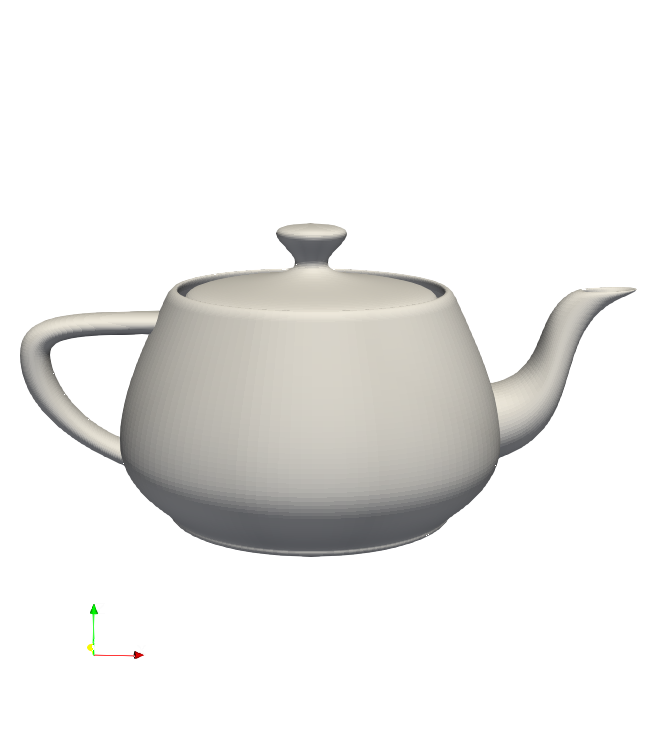
\includegraphics[width=\textwidth]{figures/teapot_geom.png}
        \caption{Teapot: 32 surface patches.}
    \end{subfigure}
    \caption{The two principal multipatch test geometries.}
    \label{fig:journal-geometries}
\end{figure}

\begin{table}[t]
    \centering
    \caption{Yeti reference problem at $(p,r)=(2,2)$.  Times exclude setup.
        A dash denotes the non-iterative direct solver.}
    \label{tab:journal-yeti-reference}
    \input{journal_results_dominance/tables/yeti_reference_table.tex}
\end{table}

Table~\ref{tab:journal-yeti-reference} provides the reference comparison.
Here $N=5760$, $\Lambda=384$, and
\eqref{eq:journal-correction-parameters} gives $q=118$.  Relative to
classical IETI-DP, the neural method reduces the count from 14 to 9 and the
solve time from $6.519$ to $4.467$ ms, reductions of $35.7\%$ and $31.5\%$,
respectively.  Direct Cholesky is faster after its factorization has been
excluded, so this is a speedup over the iterative IETI-DP baseline, not over
every method in the table.
The full refinement, degree, and patch-count studies are moved to
Appendix~\ref{app:scalability}.  Every reported Yeti point has both fewer
iterations and lower solve-only mean time than unmodified IETI-DP.

\FloatBarrier

\subsection{Target-grid retraining and projection reuse}
\label{subsec:yeti-projection-results}

Table~\ref{tab:journal-projection} tests the recommended target-grid strategy
at the three discretizations for which a $(p,r)=(2,2)$ network would require
transfer.  Each neural row uses a model trained directly at the target
$(p,r)$ and the complete calibrated preconditioner
\eqref{eq:journal-correction}.

\begin{table}[t]
    \centering
    \caption{Yeti target-grid recovery study.  Every row reports solve-only
        time and PCG iterations at tolerance $10^{-8}$; means use 50 solves and
        exclude setup.}
    \label{tab:journal-projection}
    \input{journal_results/tables/projection_table.tex}
\end{table}

At $(2,3)$, $(3,2)$, and $(4,2)$ the target-grid method needs respectively
$9$, $8$, and $10$ iterations, versus $16$, $15$, and $16$ for unmodified
IETI-DP.  Its solve-only speedups are $1.65\times$, $1.74\times$, and
$1.52\times$.  Applying the identical correction to the classical base does
not improve these three rows, so their gain is not explained by the
correction alone.

The no-retraining projector~\eqref{eq:journal-projection} remains a weaker
fallback.  In a separate audited 50-repeat control, it gives
$52.137$ ms/$16$, $9.706$ ms/$15$, and $17.068$ ms/$21$, while IETI-DP gives
$49.397$ ms/$16$, $9.372$ ms/$15$, and $13.268$ ms/$16$.  Thus projection
preserves usability at the first two targets but does not provide the
performance claim made for target-grid retraining.

\FloatBarrier

\section{Teapot and geometry generalization}
\label{sec:teapot-results}

The teapot in Figure~\ref{fig:journal-geometries}(b) is a 32-patch spline
surface in~$\R^3$.  Its patch family is included in the geometry-diverse
training distributions defined in Section~\ref{subsec:native-data}; the
principal teapot study is therefore in distribution with respect to geometry
family.  Concretely, the $(p,r)=(2,2)$ teapot rows use the 1163-operator
subdivision model, the $(2,1)$, $(2,3)$ and $(1,2)$ rows use the corresponding
103-operator models, and the $(3,2)$ and $(4,2)$ rows use the 231-operator
balanced models.  It tests solver behavior across discretizations and patch counts, not
whole-family zero-shot transfer.

\begin{table}[t]
    \centering
    \caption{Teapot reference problem at $(p,r)=(2,2)$.  Times exclude setup.
        A dash denotes the non-iterative direct solver.}
    \label{tab:journal-teapot-reference}
    \input{journal_results_dominance/tables/teapot_reference_table.tex}
\end{table}

At the reference point $N=750$, $\Lambda=256$, and $q=79$.
Table~\ref{tab:journal-teapot-reference} shows a reduction from 19 to 8
iterations and from $1.415$ to $0.700$ ms relative to classical IETI-DP,
namely $57.9\%$ and $50.5\%$.  The degree, refinement, and patch-count studies
in Appendix~\ref{app:scalability} use the same formula
\eqref{eq:journal-correction-parameters}.  Unlike the earlier local-only
models, the calibrated and residual-certified method remains below
unmodified IETI-DP at all reported teapot points.

\FloatBarrier

\subsection{What transfers across geometry?}
\label{subsec:geometry-generalization}

The principal teapot model above is in distribution, so it cannot establish
transfer to a new CAD family.  We therefore perform a stricter experiment:
the surface-diverse model of Section~\ref{subsec:native-data} is trained on
214 non-teapot patch operators, and the complete teapot family is first seen
at solver setup.  The other geometries in
Table~\ref{tab:journal-geometry-generalization} are included in that model's
training set and check that the same frozen method remains effective on its
declared distribution.  Thus only the teapot row is a whole-family neural
holdout.

Every neural row uses the complete method, including local rank-four
calibration and the interface correction
\eqref{eq:journal-correction-parameters}.  The latter is constructed from
applications of the test operator during setup.  Consequently, ``held out''
refers to the offline neural model, not to an operator-oblivious
preconditioner.  To expose how much of the gain can come from this online
adaptation, we also apply the identical correction to the classical
scaled-Dirichlet base.

\begin{table}[t]
    \centering
    \caption{Geometry recovery at $(p,r)=(2,2)$.  Each entry reports mean
        solve-only time and PCG iterations over 50 solves; setup is excluded.
        ``Held out'' means that the complete geometry family is absent from
        offline neural training.}
    \label{tab:journal-geometry-generalization}
    \input{journal_results/tables/geometry_generalization_table.tex}
\end{table}

The neural method is faster and uses fewer iterations than unmodified
IETI-DP on all six geometries.  Most importantly, on the unseen teapot it
reduces the count from 19 to 12 and the solve time from $1.392$ to
$0.979$ ms, a $1.42\times$ speedup.  On the five in-distribution geometries,
the solve-time speedup ranges from $1.23\times$ on the square to
$2.40\times$ on the 12-patch L-domain.  Figure~\ref{fig:journal-geometry-recovery}
shows the same data as ratios to unmodified IETI-DP.

This result supports whole-family transfer of the \emph{offline local model}
to the tested teapot, not distribution-free geometric generalization.  The
same-correction control is decisive for interpreting it: on the teapot, the
corrected classical base needs 6 iterations and $0.518$ ms, so the online
interface enrichment is stronger than the transferred neural base in that
case.  On the lake and the two L-domains the neural and corrected-classical
results are essentially tied.  The supported comparison is therefore with
unmodified IETI-DP; learning is not claimed to beat the strongest
identically enriched classical alternative.

\begin{figure}[t]
    \centering
    \includegraphics[width=0.94\textwidth]
    {journal_results/figures/geometry_recovery_ratios.pdf}
    \caption{Geometry-recovery ratios relative to unmodified IETI-DP; values
        below one are better.  The teapot is absent from offline neural training.
        Both enriched methods use the same test-operator-dependent interface
        correction during setup, which is excluded from the plotted solve time.}
    \label{fig:journal-geometry-recovery}
\end{figure}

\FloatBarrier

\begin{figure}[H]
    \centering
    \includegraphics[width=0.92\textwidth]
    {journal_results_dominance/figures/reference_convergence.pdf}
    \caption{Relative PCG residuals on the $(p,r)=(2,2)$ Yeti and teapot.
        Neural IETI-DP includes local rank-four calibration and the
        residual-certified correction~\eqref{eq:journal-correction-parameters};
        IETI-DP is the unmodified scaled-Dirichlet method.  Setup is excluded.}
    \label{fig:journal-reference-convergence}
\end{figure}

Figure~\ref{fig:journal-reference-convergence} shows that the gain is not a
different stopping convention: all curves start from the same iterate and are
normalized by their own initial residual.  The neural residual reaches
$10^{-8}$ after 9 rather than 14 steps on the Yeti and after 8 rather than 19
steps on the teapot.

\FloatBarrier

\subsection{Correction-rank sensitivity}
\label{subsec:rank-sensitivity}

Figure~\ref{fig:journal-rank-ablation} varies only the correction rank on the
reference discretization.  Rank $q=0$ is the native neural preconditioner
without an interface correction but retains the local calibration; the
remaining points use the same block-Krylov depth ($m=10$) and the same
residual test ($\eta_i\le0.2$) as the principal method.  Two development-stage
settings differ from the frozen rule: the sketch dimension is
$\ell_s=\min\{\Lambda,q+192\}$, without the $\lfloor\Lambda/2\rfloor$ cap, and the
local calibration caps the per-patch rank at
$\min\{4,\lceil0.125\,n_k^+\rceil,n_k^+\}$ instead of $\min\{4,n_k^+\}$.  The cap
is inactive on the 21 Yeti patches, which all keep four calibrated modes, but on
the smaller teapot skeletons it reduces the per-patch rank to two or three;
the frozen method of Section~\ref{subsec:local-model} calibrates four modes on
every patch of both reference problems.
Increasing $q$ can reduce iterations
but also adds two $\Lambda\times q$ products to every preconditioner
application.

\begin{figure}[htbp]
    \centering
    \includegraphics[width=0.92\textwidth]
    {journal_results_dominance/figures/rank_ablation.pdf}
    \caption{Development-stage neural correction-rank sensitivity at
        $(p,r)=(2,2)$.
        Both panels exclude setup; $q=0$ retains local calibration but omits the
        global correction.  Means use 20 serial solves.}
    \label{fig:journal-rank-ablation}
\end{figure}

\FloatBarrier

On the Yeti, ranks $0,39,77,116,154$ give iteration counts
$18,11,10,9,9$; solve time reaches its minimum at the tested
$q=116$.  On the teapot, ranks $0,26,52,77,103$ give
$24,13,10,8,8$ iterations, with the lower solve time again at the tested
$q=77$.  The $0.30\Lambda$ fraction is therefore the first tested fraction at
which both reference curves reach their iteration plateau; increasing the
rank further adds work without improving the count.  The final rule
\eqref{eq:journal-correction-parameters} adds a two-mode guard for endpoint
rounding, giving $q=118$ and $q=79$ on the two reference problems.

\subsection{Attribution against the same classical correction}
\label{subsec:attribution-control}

The main baseline is unmodified scaled-Dirichlet IETI-DP, as requested in the
solver comparison.  A stronger attribution question is whether the neural
local model remains preferable when the same block-Krylov construction is
applied to the classical base.  Table~\ref{tab:journal-attribution} reports
that control for every distinct configuration.

\begin{table}[p]
    \centering
    \small
    \caption{Attribution control over the complete fixed suite.  Solver cells
        report $T_{\rm solve}$ in ms / PCG iterations; setup is excluded and every
        time is a mean over 30 serial solves.  ``Same correction'' applies
        \eqref{eq:journal-correction-parameters} to classical scaled-Dirichlet
        IETI-DP.}
    \label{tab:journal-attribution}
    \input{journal_results_dominance/tables/dominance_table.tex}
\end{table}

The control is deliberately not uniformly favorable.  On most native Yeti
cases it leaves the classical count unchanged or increases it, while the
neural method remains faster.  On most teapot cases and on the largest
subdivisions, the corrected classical base is as good as or better than the
neural method.  Therefore the supported claim is strict improvement over
\emph{unmodified} IETI-DP throughout this fixed suite.  The data do not support
a claim that learning dominates the strongest identically enriched classical
alternative.

\section{Conclusions}
\label{sec:conclusions}

A geometry-conditioned SPD model alone is not sufficiently robust across this
suite.  The effective method is hybrid: the network supplies the bulk local
operator, at most four exact generalized eigenmodes calibrate each patch, and a
residual-certified block-Krylov space corrects a capped set of assembled
interface modes.  Expensive inference and adaptation are performed once and
the resulting linear operator is cached.  With one formula fixed across all
cases, the hybrid method has fewer iterations and lower solve-only mean time
than unmodified scaled-Dirichlet IETI-DP in all 16 distinct Yeti/teapot
configurations.  The observed speedup range is $1.13\times$--$2.68\times$.

These results are not evidence for a learned inverse.  No inverse of
$\Fschur$ is computed, but the setup does use exact local Schur matrices and
many matrix-free applications of $\Fschur$ and $P_0$.  The corresponding cost
is excluded from $T_{\rm solve}$, so the result applies to repeated solves
after reusable setup, not to one-right-hand-side end-to-end time.  Moreover,
the identically corrected classical control is better on most teapot cases.
The subdivision results are also enabled by subdivision examples in training;
they are not zero-shot generalization.

The evidence is limited to the constant-coefficient Poisson problem, two
principal geometries, the discretizations in~\eqref{eq:journal-pr-grid}, and
serial CPU solves.  Appropriate next tests are coefficient contrast,
distributed-memory patch solves, larger whole-family CAD holdouts, explicit
setup-amortization curves, and comparison with established adaptive
BDDC/FETI-DP coarse-space constructions.

%%%%%%%%%%%%%%%%%%%%%%%%%%%%%%%%%%%%%%%%%
%% Appendix
%%%%%%%%%%%%%%%%%%%%%%%%%%%%%%%%%%%%%%%%%
\appendix
\section{Scalability results}
\label{app:scalability}

This appendix varies one parameter at a time.  Refinement uses
$p=2$ and $r\in\{1,2,3\}$; degree uses $r=2$ and
$p\in\{1,2,3,4\}$; patch scaling fixes $(p,r)=(2,2)$.  Every point reports
both solve-only time and iterations for the requested methods.  Direct
Cholesky appears only in the timing panel because it has no iteration count.
In the patch-count sweeps, the Yeti model
at $K=21$ is the fixed-patch specialist, while the subdivided Yeti points and
all three teapot points -- including the unsubdivided $K=32$ reference -- use
the declared 1163-operator subdivision model.  The patch-count
sweeps therefore test solver scaling inside that augmented training
distribution; they do not test zero-shot transfer to child patches.

\subsection{Yeti}

Across $r=1,2,3$ at $p=2$, neural IETI-DP uses 8, 9, and 9 iterations,
compared with 12, 14, and 16 for classical IETI-DP.  At $r=2$ and
$p=1,2,3,4$, the corresponding counts are 10, 9, 8, and 10 versus 13, 14,
15, and 16.  At $K=21,84,336$, the neural counts are 9, 12, and 15 versus
14, 19, and 21; see Figures~\ref{fig:journal-yeti-refinement},
\ref{fig:journal-yeti-degree} and~\ref{fig:journal-yeti-patches}.
The narrowest Yeti time margin occurs at $(p,r)=(1,2)$:
$2.521$ ms versus $3.079$ ms, a $1.22\times$ speedup; the largest patch count
$K=336$ is next, at $54.177$ ms versus $69.192$ ms, a $1.28\times$ speedup.

\begin{figure}[p]
    \centering
    \includegraphics[width=\textwidth]
    {journal_results_dominance/figures/yeti_refinement_scalability.pdf}
    \caption{Yeti refinement study at $p=2$, $K=21$: solve-only time and
        iterations for all five methods.  Neural IETI-DP uses
        \eqref{eq:journal-correction-parameters}; setup is excluded.}
    \label{fig:journal-yeti-refinement}
\end{figure}

\begin{figure}[p]
    \centering
    \includegraphics[width=\textwidth]
    {journal_results_dominance/figures/yeti_degree_scalability.pdf}
    \caption{Yeti degree study at $r=2$, $K=21$: solve-only time and
        iterations for all five methods; setup is excluded.}
    \label{fig:journal-yeti-degree}
\end{figure}

\begin{figure}[p]
    \centering
    \includegraphics[width=\textwidth]
    {journal_results_dominance/figures/yeti_patches_scalability.pdf}
    \caption{Yeti patch-count study at $(p,r)=(2,2)$: solve-only time and
        iterations for all five methods.  The $K=84,336$ neural points use the
        subdivision-augmented model; setup is excluded.}
    \label{fig:journal-yeti-patches}
\end{figure}

\subsection{Teapot}

At $p=2$, the neural counts for $r=1,2,3$ are 10, 8, and 7, versus 15, 19,
and 22 for classical IETI-DP.  At $r=2$, the neural degree counts for
$p=1,2,3,4$ are 7, 8, 17, and 17 versus 16, 19, 21, and 23.  The smallest
time margin is the high-degree case $p=3$: $1.955$ ms versus $2.216$ ms,
or $1.13\times$.  At $K=32,128,512$, the neural counts are 8, 10, and 22
versus 19, 24, and 36, with solve-only speedups $2.02\times$,
$2.16\times$, and $1.54\times$, respectively; see
Figures~\ref{fig:journal-teapot-refinement},
\ref{fig:journal-teapot-degree} and~\ref{fig:journal-teapot-patches}.

\begin{figure}[p]
    \centering
    \includegraphics[width=\textwidth]
    {journal_results_dominance/figures/teapot_refinement_scalability.pdf}
    \caption{Teapot refinement study at $p=2$, $K=32$: solve-only time and
        iterations for all five methods; setup is excluded.}
    \label{fig:journal-teapot-refinement}
\end{figure}

\begin{figure}[p]
    \centering
    \includegraphics[width=\textwidth]
    {journal_results_dominance/figures/teapot_degree_scalability.pdf}
    \caption{Teapot degree study at $r=2$, $K=32$: solve-only time and
        iterations for all five methods; setup is excluded.}
    \label{fig:journal-teapot-degree}
\end{figure}

\begin{figure}[p]
    \centering
    \includegraphics[width=\textwidth]
    {journal_results_dominance/figures/teapot_patches_scalability.pdf}
    \caption{Teapot patch-count study at $(p,r)=(2,2)$: solve-only time and
        iterations for all five methods.  The neural model includes subdivided
        teapot patches in training; setup is excluded.}
    \label{fig:journal-teapot-patches}
\end{figure}

\FloatBarrier

%%%%%%%%%%%%%%%%%%%%%%%%%%%%%%%%%%%%%%%%%
%% Bibliography (Harvard notation)
%%%%%%%%%%%%%%%%%%%%%%%%%%%%%%%%%%%%%%%%%
\clearpage
\begin{thebibliography}{99}
    \bibitem{george1973nested}
    George, J.A., 1973. Nested dissection of a regular finite element mesh. SIAM Journal on Numerical Analysis, 10(2), pp.345--363.

    \bibitem{hackbusch1994iterative}
    Hackbusch, W., 1994. Iterative solution of large sparse systems of equations. Springer-Verlag, New York.

    \bibitem{saad2003iterative}
    Saad, Y., 2003. Iterative methods for sparse linear systems (2nd edn.). SIAM, Philadelphia.

    \bibitem{van2003iterative}
    Van der Vorst, H.A., 2003. Iterative Krylov methods for large linear systems (No. 13). Cambridge University Press.

    \bibitem{kleiss2012ieti}
    Kleiss, S.K., Pechstein, C., Jüttler, B. and Tomar, S., 2012. IETI–isogeometric tearing and interconnecting. Computer methods in applied mechanics and engineering, 247, pp.201-215.

    \bibitem{schneckenleitner2020condition}
    Schneckenleitner, R. and Takacs, S., 2020. Condition number bounds for IETI-DP methods that are explicit in $h$ and $p$. Mathematical Models and Methods in Applied Sciences, 30(11), pp.2067--2103.

    \bibitem{farhat1991method}
    Farhat, C. and Roux, F.X., 1991. A method of finite element tearing and interconnecting and its parallel solution algorithm. International Journal for Numerical Methods in Engineering, 32(6), pp.1205-1227.

    \bibitem{hofer2018dual}
    Hofer, C. and Langer, U., 2017. Dual-primal isogeometric tearing and interconnecting solvers for multipatch dG-IgA equations. Computer Methods in Applied Mechanics and Engineering, 316, pp.2-21.

    \bibitem{pechstein2013finite}
    Pechstein, C., 2013. Finite and boundary element tearing and interconnecting solvers for multiscale problems. Lecture Notes in Computational Science and Engineering, Vol. 90. Springer.

    \bibitem{wu2026dlhim}
    Wu, Y., van Beek, J.W., Dolean, V. and Heinlein, A., 2026. Are Deep Learning Based Hybrid PDE Solvers Reliable? Why Training Paradigms and Update Strategies Matter. arXiv preprint arXiv:2602.06842.

    \bibitem{Lynch1964}
    Lynch, R.E., Rice, J.R. and Thomas, D.H., 1964. Direct solution of partial difference equations by tensor product methods. Numerische Mathematik, 6(1), pp.185-199.

    \bibitem{de2011geopdes}
    De Falco, C., Reali, A. and Vázquez, R., 2011. GeoPDEs: a research tool for isogeometric analysis of PDEs. Advances in Engineering Software, 42(12), pp.1020-1034.

    \bibitem{de1978practical}
    De Boor, C. and De Boor, C., 1978. A practical guide to splines (Vol. 27, p. 325). New York: springer.

    \bibitem{fanaskov2023spectral}
    Fanaskov, V.S. and Oseledets, I.V., 2023, December. Spectral neural operators. In Doklady Mathematics (Vol. 108, No. Suppl 2, pp. S226-S232). Moscow: Pleiades Publishing.

    \bibitem{montardini2025isogeometric}
    Montardini, M., Takacs, S. and Tani, M., 2025. The Isogeometric Fast Fourier-based Diagonalization method. arXiv preprint arXiv:2512.20269.

    \bibitem{cottrell2009isogeometric}
    Cottrell, J.A., Hughes, T.J. and Bazilevs, Y., 2009. Isogeometric analysis: toward integration of CAD and FEA. John Wiley $\&$ Sons.

    \bibitem{adler2010geometry}
    Adler, R.J., 2010. The geometry of random fields. Society for Industrial and Applied Mathematics.

    \bibitem{saad1993flexible}
    Saad, Y., 1993. A flexible inner-outer preconditioned GMRES algorithm. SIAM Journal on Scientific Computing, 14(2), pp.461-469.

    \bibitem{ghiotto2025hypernos}
    Ghiotto, M., 2025. HyperNOs: automated and parallel library for neural operators research. Bollettino dell'Unione Matematica Italiana, pp.1-35.

    \bibitem{srivastava2014dropout}
    Srivastava, N., Hinton, G., Krizhevsky, A., Sutskever, I. and Salakhutdinov, R., 2014. Dropout: a simple way to prevent neural networks from overfitting. The journal of machine learning research, 15(1), pp.1929-1958.

    \bibitem{math10214014}
    Cui, C., Jiang, K., Liu, Y. and Shu, S., 2022. Fourier neural solver for large sparse linear algebraic systems. Mathematics, 10(21), p.4014.

    \bibitem{vaswani2017attention}
    Vaswani, A., Shazeer, N., Parmar, N., Uszkoreit, J., Jones, L., Gomez, A.N., Kaiser, Ł. and Polosukhin, I., 2017. Attention is all you need. Advances in neural information processing systems, 30.

    \bibitem{he2016identity}
    He, K., Zhang, X., Ren, S. and Sun, J., 2016, September. Identity mappings in deep residual networks. In European conference on computer vision (pp. 630-645). Cham: Springer International Publishing.

    \bibitem{he2016deep}
    He, K., Zhang, X., Ren, S. and Sun, J., 2016. Deep residual learning for image recognition. In Proceedings of the IEEE conference on computer vision and pattern recognition (pp. 770-778).

    \bibitem{kahana2023geometry}
    Kahana, A., Zhang, E., Goswami, S., Karniadakis, G., Ranade, R. and Pathak, J., 2023. On the geometry transferability of the hybrid iterative numerical solver for differential equations. Computational Mechanics, 72(3), pp.471-484.

    \bibitem{kopanivcakova2025deeponet}
    Kopaničáková, A. and Karniadakis, G.E., 2025. Deeponet based preconditioning strategies for solving parametric linear systems of equations. SIAM Journal on Scientific Computing, 47(1), pp.C151-C181.

    \bibitem{brenner2008mathematical}
    Brenner, S.C. and Scott, L.R., 2008. The mathematical theory of finite element methods. New York, NY: Springer New York.

    \bibitem{sampath2010parallel}
    Sampath, R.S. and Biros, G., 2010. A parallel geometric multigrid method for finite elements on octree meshes. SIAM Journal on Scientific Computing, 32(3), pp.1361-1392.

    \bibitem{lee2025hybrid}
    Lee, Y., Florencio, F.L., Pathak, J. and Karniadakis, G.E., 2025. Hybrid Iterative Solvers with Geometry-Aware Neural Preconditioners for Parametric PDEs. arXiv preprint arXiv:2512.14596.

    \bibitem{chen1995universal}
    Chen, T. and Chen, H., 1995. Universal approximation to nonlinear operators by neural networks with arbitrary activation functions and its application to dynamical systems. IEEE transactions on neural networks, 6(4), pp.911-920.

    \bibitem{hughes2005isogeometric}
    Hughes, T.J., Cottrell, J.A. and Bazilevs, Y., 2005. Isogeometric analysis: CAD, finite elements, NURBS, exact geometry and mesh refinement. Computer methods in applied mechanics and engineering, 194(39-41), pp.4135-4195.

    \bibitem{hendrycks2016gaussian}
    Hendrycks, D. and Gimpel, K., 2016. Gaussian error linear units (gelus). arXiv preprint arXiv:1606.08415.

    \bibitem{watanabe2023tree}
    Watanabe, S., 2023. Tree-structured parzen estimator: Understanding its algorithm components and their roles for better empirical performance. arXiv preprint arXiv:2304.11127.

    \bibitem{bergstra2015hyperopt}
    Bergstra, J., Komer, B., Eliasmith, C., Yamins, D. and Cox, D.D., 2015. Hyperopt: a python library for model selection and hyperparameter optimization. Computational Science $\&$ Discovery, 8(1), p.014008.

    \bibitem{li2020massivelyparallelhyperparametertuning}
    Li, L., Jamieson, K., Rostamizadeh, A., Gonina, E., Ben-Tzur, J., Hardt, M., Recht, B. and Talwalkar, A., 2020. A system for massively parallel hyperparameter tuning. Proceedings of machine learning and systems, 2, pp.230-246.

    \bibitem{loshchilov2019decoupledweightdecayregularization}
    Loshchilov, I. and Hutter, F., 2017. Decoupled weight decay regularization. arXiv preprint arXiv:1711.05101.

    \bibitem{sangalli2016isogeometric}
    Sangalli, G. and Tani, M., 2016. Isogeometric preconditioners based on fast solvers for the Sylvester equation. SIAM Journal on Scientific Computing, 38(6), pp.A3644-A3671.

    \bibitem{gahalaut2019condition}
    Gahalaut, K.P., Tomar, S.K. and Douglas, C., 2014. Condition number estimates for matrices arising in NURBS based isogeometric discretizations of elliptic partial differential equations. arXiv preprint arXiv:1406.6808.

    \bibitem{trottenberg2000multigrid}
    Trottenberg, U., Oosterlee, C.W. and Schuller, A., 2001. Multigrid methods. Academic press.

    \bibitem{toselli2004domain}
    Toselli, A. and Widlund, O., 2004. Domain decomposition methods-algorithms and theory (Vol. 34). Springer Science $\&$ Business Media.

    \bibitem{lu2021learning}
    Lu, L., Jin, P., Pang, G., Zhang, Z. and Karniadakis, G.E., 2021. Learning nonlinear operators via DeepONet based on the universal approximation theorem of operators. Nature machine intelligence, 3(3), pp.218-229.

    \bibitem{li2021fourier}
    Li, Z., Kovachki, N., Azizzadenesheli, K., Liu, B., Bhattacharya, K., Stuart, A. and Anandkumar, A., 2020. Fourier neural operator for parametric partial differential equations. arXiv preprint arXiv:2010.08895.

    \bibitem{rahaman2019spectral}
    Rahaman, N., Baratin, A., Arpit, D., Draxler, F., Lin, M., Hamprecht, F., Bengio, Y. and Courville, A., 2019, May. On the spectral bias of neural networks. In International conference on machine learning (pp. 5301-5310). PMLR.

    \bibitem{tielen2020pmultigrid}
    Tielen, R.P.W.M., Möller, M., Göddeke, D. and Vuik, C., 2020. p-multigrid methods and their comparison to h-multigrid methods within Isogeometric Analysis. Computer Methods in Applied Mechanics and Engineering, 372, p.113347.

    \bibitem{donatelli2015robust}
    Donatelli, M., Garoni, C., Manni, C., Serra-Capizzano, S. and Speleers, H., 2015. Robust and optimal multi-iterative techniques for IgA Galerkin linear systems. Computer Methods in Applied Mechanics and Engineering, 284, pp.230--264.

    \bibitem{hofreither2017robust}
    Hofreither, C. and Takacs, S., 2017. Robust multigrid for isogeometric analysis based on stable splittings of spline spaces. SIAM Journal on Numerical Analysis, 55(4), pp.2004--2024.

    \bibitem{dede2015isogeometric}
    Dedè, L. and Quarteroni, A., 2015. Isogeometric analysis for second order partial differential equations on surfaces. Computer Methods in Applied Mechanics and Engineering, 284, pp.807--834.

    \bibitem{dziuk2013finite}
    Dziuk, G. and Elliott, C.M., 2013. Finite element methods for surface PDEs. Acta Numerica, 22, pp.289--396.

    \bibitem{moller2026iganet}
    Möller, M., Obermair, G., Singer, I., Gollmann, C., Reali, A. and Elgeti, S., 2026. IGANets: Isogeometric analysis networks and their applications to linear structural analysis problems. Engineering with Computers, 42(3), p.102.

    \bibitem{karniadakis2025nonlinearprec}
    Lee, Y., Liu, S., Darbon, J. and Karniadakis, G.E., 2025. A Neural-Operator Preconditioned Newton Method for Accelerated Nonlinear Solvers. arXiv preprint arXiv:2511.08811.

    \bibitem{karniadakis2025nspod}
    Levrero-Florencio, F., Lee, Y., Pathak, J. and Karniadakis, G.E., 2026. NSPOD: acceleratingthe convergence ofKrylov-based iterative linearsolvers via approximated PODs. arXiv preprint arXiv:2605.07828.

\end{thebibliography}
% \printbibliography

\end{document}
